\phantomsection
\addcontentsline{toc}{section}{Quantum Approach}
\section*{Quantum Approach}

\phantomsection
\addcontentsline{toc}{subsection}{Benefits of a Quantum Approach}
\subsection*{Benefits of a Quantum Approach}

\phantomsection
\addcontentsline{toc}{subsubsection}{Parallelisation}
\subsubsection*{Parallelisation}
A lot of the speed-ups from quantum computing relies on quantum parallelism, which arises from the ability for a quantum register (simply a place where qubits are stored) to exist in the superposition of base states. Applying a function/gate is performed on each of the components of the superposition, but due to the register being in a superposition, the function is only applied one time. The number of possible states is $2^{n}$, with n being the number of qubits in the register. Therefore, you can perform one operation on a quantum computer that would take an exponential number of operations on a classical computer.

For example, take the function (1), applied over a quantum register in an equally weighted superposition of the states 0 through 6, represented by $Q: \{0, 1, 2, 3, 4, 5, 6\}$:

\begin{align}
	f(x)          & = x^{2}+1                 \\
	\implies f(Q) & = \{1, 2, 5, 10, 26, 37\}
\end{align}

Although we have only performed the function once, every single component of the superposition has had the function applied to it. To perform the same operation on a classical computer, on the same data would require iterating over each element and performing the function on each number, 0 through 6, taking n iterations to complete, n being the number of elements performing the operation on.

However, as we increase the number of superposition states, we decrease the change that, upon measuring the quantum register and hence collapsing the superposition of states, that the desired value is measured. However, quantum algorithms can be designed to use properties of the output as a whole, not just a particular one.

This parallelism therefore can be utilised to speed up many problems and algorithms that, whilst possible on a classical system, would take a very large amount of time as the size of the problem increases.

\phantomsection
\addcontentsline{toc}{subsubsection}{Quantum Algorithms}
\subsubsection*{Quantum Algorithms}

\phantomsection
\addcontentsline{toc}{paragraph}{Defining Complexity}
\paragraph*{Defining Complexity}
\noindent
Algorithms and problems can be sorted into different complexities, which help one understand what problems can be efficiently solved, and the time and space their solutions take up. In \autoref{fig:Complexity Theory Classes}, we can see the relation between each class. P and NL are the two classes where problems can be solved in polynomial time, and a general rule of thumb is that any solution in these two classes can be efficiently solved and are tractable.

Quantum Algorithms, when properly designed, can exist outside of this P-complexity space, referred to as BQP (Bounded Quantum Polynomial). This contains any solution to a problem that can be solved in polynomial time on a quantum computer, but not a classical computer. \cite{doi:10.1137/S0097539796300921}

\begin{figure}
	\begin{figure}[H]
		\centering
		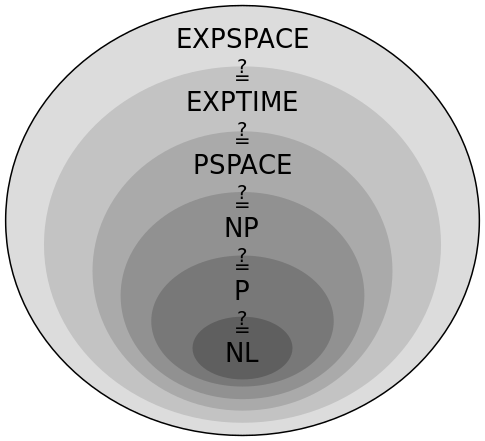
\includegraphics[width=0.4\textwidth]{Complexity_subsets_pspace.png}
		\caption{Complexity Theory Classes \cite{complexity}}
		\label{fig:Complexity Theory Classes}
	\end{figure}

\end{figure}

For example, integer factorisation. This is relied upon for many cryptography systems, such as RSA public-key encryption. RSA keys are composed of two semiprimes, numbers that are the product of two prime numbers. Whilst it has not yet been proven that the factorisation of prime integers is not a P-complexity space problem, the best publicly available algorithm currently has a time complexity of

\begin{align}
	O(\exp((\sqrt[3]{\frac{64}{9}}+o(1))(\ln{n})^{\frac{1}{3}}(\ln\ln{n})^{\frac{2}{3}}))
\end{align}
\noindent
for n number of bits. Whilst this is sub exponential, and therefore not in EXPTIME-complexity space, it does significantly exceed polynomial time. \cite{10.5555/270146}

\phantomsection
\addcontentsline{toc}{paragraph}{Shor's Algorithm}
\paragraph*{Shor's Algorithm}
\noindent
There is however, an algorithm devised by Peter Shor, which, using a quantum computer, can factorise large prime integers in polynomial time \cite{365700}.

\begin{align}
	O((\log{n})^{2}(\log\log{n}))
\end{align}

\noindent
This algorithm was first implemented in 2001, using a 7 qubit NMR quantum computer \cite{Vandersypen_2001}.
This is just one example of a problem that can be significantly sped up by designing quantum algorithms. If this algorithm can be scaled up, it provides a significant threat to cryptography.

\phantomsection
\addcontentsline{toc}{paragraph}{Differential Equation solvers}
\paragraph*{Differential Equation solvers}
\noindent
Many, if not all mathematical and scientific models are underpinned by differential equations. They are used to describe how functions interact with their derivative and change in relation to other variables. Some common differential equations include:

\begin{align}
	\frac{d^{2}u}{du^{2}}+\omega^{2} u                                                                                                    & = 0 &  & \text{Describing a harmonic oscillator}                 \\[0.5em]
	L\frac{d^{2}}{du^{2}}+g\sin{u}                                                                                                        & = 0 &  & \text{Describing the motion of a pendulum, length L}    \\[0.5em]
	\nabla^{2}f(x, y, z) = \frac{\partial^{2}f}{\partial x^{2}}+\frac{\partial^{2}f}{\partial y^{2}}+\frac{\partial^{2}f}{\partial z^{2}} & = 0 &  & \text{3-dimensional Laplace equation \cite{laplace_eq}}
\end{align}

\noindent
The speed with which we can either, find a solution to a differential equation (that is, find functions that represent each of the variables involved), or find a numeric solution to the differential equation, therefore plays a large role in the speed that we can model biological systems.

For both linear (the system only contains linear equations of u and it's derivatives), and non-linear (system contains non-linear functions of u and it's derivatives) differential equations, there exists quantum algorithms for solving both. Classical algorithms for solving differential equations typically grow exponentially with the number of variables involved. However, using quantum algorithms this can be reduced to poly-logarithmic time or better \cite{10.48550/arxiv.2011.06571,10.48550/arxiv.0812.4423}, and for linear differential equations, even to quadratic time ($O(n^{2})$) \cite{Berry_2014}.


\phantomsection
\addcontentsline{toc}{paragraph}{Fast Fourier Transform}
\paragraph*{Fast Fourier Transform}
\noindent
The Fourier Transform is a mathematical transform that decomposes a function into it's frequency components. For example, splitting a musical waveform into the intensity of the individual pitches and harmonics. However, it has many uses, including solving partial differential equations.

The Fast Fourier Transform (FFT) was (re)discovered by James Cooley and John Turkey in 1965, thought the be an original discovery at the time, but it was later found that Carl Gauss had already devised it over 160 years earlier \cite{cooley_tukey_1965}. This algorithm was pivotal in a giant number of fields, reducing the time complexity to perform a Fourier transform from $O(n^{2})$ to $O(n\log{n})$. In \autoref{fig:FFTcompare} it is clear that the FFT scales much more slowly than traditional methods, as the dimensions of the input matrix increases.

\begin{figure}[H]
	\centering
	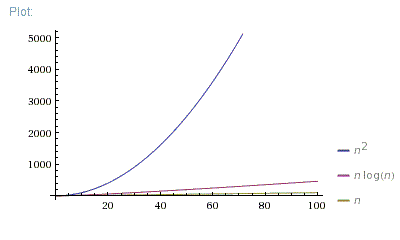
\includegraphics[width=0.58\textwidth]{PB0M1.png}
	\caption{$O(n^{2})$ vs $O(n\log{n})$ vs $O(n)$}
	\label{fig:FFTcompare}
\end{figure}

\phantomsection
\addcontentsline{toc}{paragraph}{Quantum Fast Fourier Transform}
\paragraph*{Quantum Fast Fourier Transform}
\noindent
A quantum algorithm also exists to perform an FFT on a quantum system, and when implemented properly can scale at $O(n)$ \cite{asaka_sakai_yahagi_2020, Quantum-assisted}. See \autoref{fig:FFTcompare} \\ \\

\noindent
The exponential speed up - along with the quantum parallelism discussed earlier - provided by quantum algorithms can vastly increase the speed and efficiency that we can simulate biological systems with, especially as the number of variables and particles simulated grows.

\phantomsection
\addcontentsline{toc}{subsection}{Drawbacks of a Quantum Approach}
\subsection*{Drawbacks of a Quantum Approach}
Whilst this paints a rather favourable picture for quantum computing matching and superseding HPC in the field of computational biology, there exists a number of significant drawbacks.

\phantomsection
\addcontentsline{toc}{subsubsection}{Quantum Effects}
\subsubsection*{Quantum Effects}
Whilst quantum computing as a concept has been around for over 4 decades, the actual capabilities to construct and maintain quantum computers have only come to fruition recently, with huge corporations and small start-ups producing systems using various designs. However, regardless of the design philosophy used in a quantum computer, it is still very difficult to maintain the entanglement of many qubits at once, and this only becomes more difficult as the number of qubits increases. Entanglement of qubits is critical to many quantum gates functioning. The greater the number of entanglement qubits, the greater the number of states that computer can represent and be in a superposition of.

Additionally, qubits need to be entangled with each other, but not entangled with anything else; They must be designed very carefully not to entangle with any other physical system and therefore become decoherent.

Qubits must also be shielded from any kind of interferences, such as radiation or other particles. Some decoherence and noise is inevitable in any quantum system, however our techniques to manage these factors are relatively immature and limit the ability to scale quantum systems. For example, we can create a "logical" qubit that is composed of many entangled qubits to represent one noise-free qubit. However, it is estimated that 100 to 1000 physical qubits are required to create one logical qubit, which brings us back to the issue of maintaining coherence between qubits.

Qubits are not just isolated units. Quantum computers need to be able to control and measure each qubit's state, requiring large amounts of circuitry, and this increases linearly as the number of qubits increases. If using a logical qubit system, this would exacerbate this issue even more.

Decoherence limits the amount of time we can run quantum computers for before the error rate becomes too high to take any meaningful reading. If we wanted to simulate a biological system that acts over a couple of days, then we would currently have significant challenge maintaining coherence during that timescale.

\phantomsection
\addcontentsline{toc}{subsubsection}{Cost}
\subsubsection*{Cost}
Whilst the construction of quantum computers is not cheap - Dwave's 2000 qubit quantum computer has a price tag of \$15 million, it is the cooling and power requirements of quantum systems that really increases the cost.

\phantomsection
\addcontentsline{toc}{paragraph}{Cooling}
\paragraph*{Cooling}
\noindent
Qubits must be cooled to temperatures just above absolute zero in order to reduce the effect of heat radiation, and also to stabilise the qubit. In quantum systems that use superconducting magnets, cooling is also required for those magnets to superconduct. Cooling lasers are used to freeze qubits and held, whist being manipulated and measured using other qubits.
The costs are due to the high energy requirements of these lasers, and cost of supercooled fluids like Helium.

\phantomsection
\addcontentsline{toc}{subsubsection}{Classical Processing}
\subsubsection*{Classical Processing}
Whilst many quantum algorithms can provide exponential speed-ups over classical equivalents, many of these algorithms require additionally processing, either via another quantum algorithm or via processing on a classical system. This is due to qubits being superposed, and the need for individual state's probabilities needing to be measured. This post-processing can actually nullify the benefits one gains when running quantum algorithms, and can even make some algorithms scale worse than their classical counterparts. 

Additionally, the scaling of a quantum algorithm does not show the whole picture. Whilst in theory a quantum algorithm may scale more efficiently that a classical equivalent, it does not mean that the specific implementation of a quantum computer can complete the computation quicker than a classical computer.
